%!TEX encoding = UTF-8 Unicode
%!TEX root = ../algos-geometriques.tex


\chapter{Cercle}

Un cercle est caractérisé par son centre et son rayon. C'est un type qui n'existe pas en Cocoa, il est défini dans \texttt{ElCanari} par une structure non mutable. Ce type est implémenté dans \texttt{GeometricCircle.swift}. Il est simplement construit à partir d'un point et d'un rayon.

\begin{lstlisting}
struct GeometricCircle {
  let center : CGPoint
  let radius : CGFloat

  init (center : CGPoint, radius : CGFloat) {
    self.center = center
    self.radius = radius
  }
}
\end{lstlisting}





\section{Intersection entre deux cercles}

Élémentaire, il y a intersection si la distance entre les centres est inférieure ou égale à la somme des rayons.


\begin{lstlisting}
  func intersects (circle : GeometricCircle) -> Bool {
    let d = CGPoint.distance (self.center, circle.center)
    return d <= (self.radius + circle.radius)
  }
\end{lstlisting}






\section{Intersection avec un segment}

Voici quelques illustrations des différents cas :
\begin{center}
  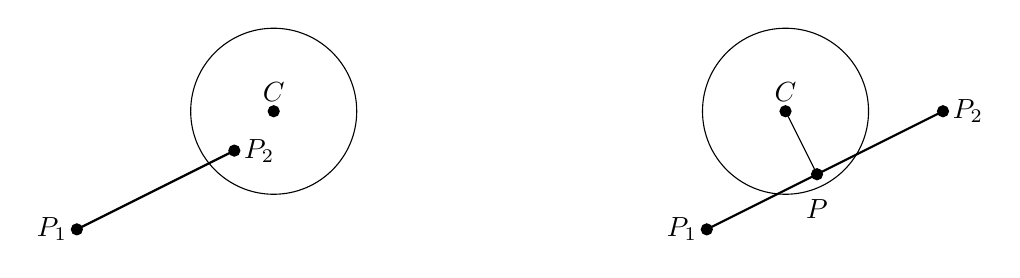
\begin{tikzpicture}
    \draw (0, 0) -- (2, 1) ;
    \draw[thick] (0, 0) -- (2, 1) ;
    \draw[fill] (0, 0) circle (2pt) ;
    \draw[fill] (2, 1) circle (2pt) ;
    \draw[left] (0, 0) node {$P_1$} ;
    \draw[above] (2.5, 1.5) node {$C$} ;
    \draw (2.5, 1.5) circle (30pt) ;
    \draw[fill] (2.5, 1.5) circle (2pt) ;
    \draw[right] (2, 1) node {$P_2$} ;
    \begin{scope}[xshift=8cm]
      \draw[thick] (0, 0) -- (3, 1.5) ;
      \draw[fill] (0, 0) circle (2pt) ;
      \draw[fill] (3, 1.5) circle (2pt) ;
      \draw[left] (0, 0) node {$P_1$} ;
      \draw[above] (1, 1.5) node {$C$} ;
      \draw (1, 1.5) circle (30pt) ;
      \draw[fill] (1, 1.5) circle (2pt) ;
      \draw[right] (3, 1.5) node {$P_2$} ;
      \draw (1, 1.5) -- (1.4, .7) ;
      \draw[fill] (1.4, .7) circle (2pt) ;
      \draw[below] (1.4, .5) node {$P$} ;
    \end{scope}
  \end{tikzpicture}
\end{center}

On va calculer l'abscisse du point $P$, projection de $C$ sur $P_1P_2$ :
\begin{itemize}
  \item pour simplifier, on translate les points de façon à amener $P_1$ en $(0, 0)$ ;
  \item l'abscisse curviligne de $P$ est repérée par $\mu$ ($\mu = 0$, $P$ est en $P_1$, $\mu = 1$, $P$ est en $P_2$).
\end{itemize}
Les coordonnées de $P_2$ sont donc : $(p2x, p2y)$, celles de $P$ $(\mu\cdot p2x, \mu\cdot p2y)$, et celles de $C$ $(Cx, Cy)$.

Le point $P$ est défini par $\overrightarrow{P_1P_2}~.~\overrightarrow{PC} = 0$, donc :
\begin{equation*}
p2x \cdot (\mu\cdot p2x - Cx) + p2y \cdot (\mu\cdot p2y - Cy) = 0
\end{equation*}

D'où :
\begin{equation*}
\mu = \frac{p2x \cdot Cx+ p2y \cdot Cy}{p2x^2 + p2y^2}
\end{equation*}

Si $\mu < 0$ ou $\mu > 1$, le point $P$ est en dehors du segment, il n'y a pas d'intersection. Sinon, on calcule la distance entre $P$ et $C$ :
\begin{equation*}
d_{PC} = \sqrt{(\mu\cdot p2x - Cx)^2 + (\mu\cdot p2y - Cy)^2}
\end{equation*}

Et il y a intersection si $d_{PC} \leqslant radius$.


\begin{lstlisting}
  func intersects (segmentFrom inP1 : NSPoint, to inP2 : NSPoint) -> Bool {
  //--- We translate P1, P2, C (center of circle) so that P1 is at (0, 0)
    let p2x = inP2.x - inP1.x
    let p2y = inP2.y - inP1.y
    let Cx = self.center.x - inP1.x
    let Cy = self.center.y - inP1.y
  //--- Then we compute the relative abscisse \textmu of P, the projection of C on P1P2
    let \textmu = (p2x * Cx + p2y * Cy) / (p2x * p2x + p2y * p2y)
    if \textmu < 0.0 { // Outside
      return false
    }else if \textmu > 1.0 { // Outside
      return false
    }else{ // Inside: we compute the distance between P and C
      let dx = \textmu * p2x - Cx
      let dy = \textmu * p2y - Cy
      let d = (dx * dx + dy * dy).squareRoot ()
      return d <= self.radius
    }
  }
\end{lstlisting}


\section{Intersection avec un segment (ancien)}

{\bf Ancien algorithm.} L'intersection entre un cercle et un segment est plus compliquée, il y a plusieurs tests à faire :
\begin{itemize}
\item d'abord, on teste si la distance entre le centre du cercle et les extrémités du segment ; si l'une de ces distances est inférieure au rayon du cercle, il y a intersection ;
\item ensuite, on calcule les coordonnées du centre du cercle dans le repère dont l'origine est le centre du segment, et l'axe des abscisses la direction du segment ; il y a intersection si et seulement si :
  \begin{itemize}
  \item la valeur absolue de l'ordonnée du centre est inférieure au rayon ;
  \item la valeur absolue de l'abscisse du centre est inférieure à la moitié de la distance entre les deux points.
  \end{itemize}
\end{itemize}

\begin{center}
  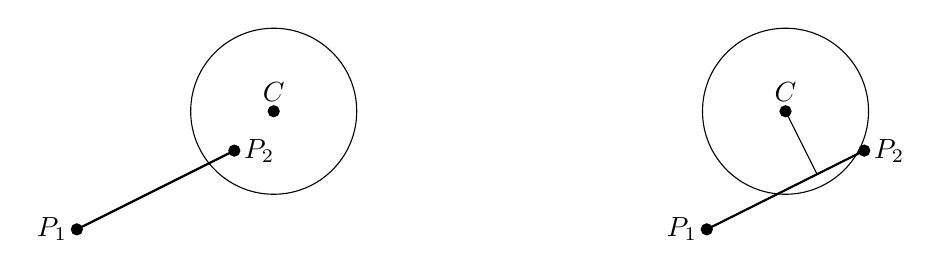
\begin{tikzpicture}
    \draw (0, 0) -- (2, 1) ;
    \draw[thick] (0, 0) -- (2, 1) ;
    \draw[fill] (0, 0) circle (2pt) ;
    \draw[fill] (2, 1) circle (2pt) ;
    \draw[left] (0, 0) node {$P_1$} ;
    \draw[above] (2.5, 1.5) node {$C$} ;
    \draw (2.5, 1.5) circle (30pt) ;
    \draw[fill] (2.5, 1.5) circle (2pt) ;
    \draw[right] (2, 1) node {$P_2$} ;
    \begin{scope}[xshift=8cm]
      \draw (0, 0) -- (2, 1) ;
      \draw[thick] (0, 0) -- (2, 1) ;
      \draw[fill] (0, 0) circle (2pt) ;
      \draw[fill] (2, 1) circle (2pt) ;
      \draw[left] (0, 0) node {$P_1$} ;
      \draw[above] (1, 1.5) node {$C$} ;
      \draw (1, 1.5) circle (30pt) ;
      \draw[fill] (1, 1.5) circle (2pt) ;
      \draw[right] (2, 1) node {$P_2$} ;
      \draw (1, 1.5) -- (1.4, .7) ;
    \end{scope}
  \end{tikzpicture}
\end{center}


\begin{lstlisting}
  func intersects (segmentFrom p1 : CGPoint, to p2 : CGPoint) -> Bool {
    var intersects = CGPoint.distance (p1, self.center) <= self.radius
    if !intersects {
      intersects = CGPoint.distance (p2, self.center) <= self.radius
    }
    if !intersects {
      let segmentAngle = CGPoint.angleInRadian (p1, p2)
      let segmentCenter = CGPoint (x: (p1.x + p2.x) / 2.0, y: (p1.y + p2.y) / 2.0)
      let tr = CGAffineTransform (rotationAngle: -segmentAngle)
              .translatedBy (x:-segmentCenter.x, y:-segmentCenter.y)
      let point = self.center.applying (tr)
      intersects = abs (point.y) <= self.radius
      if intersects {
        let segmentLength = CGPoint.distance (p1, p2)
        intersects = abs (point.x) <= (segmentLength * 0.5)
      }
    }
    return intersects
  }
\end{lstlisting}

